\section{Introducción Teórica}

\subsection{PageRank}

PageRank es un algoritmo que modela un proceso aleatorio de navegación a través de
distintas páginas Web, cuyo objetivo es generar un ranking de importancia de páginas,
que en la práctica se utiliza para refinar los resultados de búsquedas de texto en las mismas
para refinar los resultados por relevancia.

El problema se define como encontrar el autovector asociado al autovalor 1 de la matriz de transiciones
correspondientes a un grafo de páginas Web interconectadas. Dado que esta matriz se puede ajustar
para que sea estocástica, el autovector corresponde a la proporción de tiempo que pasa un navegante
aleatorio en una página, que en la realidad resulta un buen indicador de importancia.

La manera en cómo se modela el problema del ranking es usando una matriz de adyacencias.
Sea $W \in \mathbb{R}^{n \times n}$ donde $n$ es la cantidad de sitios indexados, luego el elemento
$w_{ij}$ es igual $1$ si existe un link de la página $i$ a la página $j$ y $0$ en caso
contrario. A su vez los links autoreferenciados se ignoran por lo que en diagonal tenemos todos valores nulos.

Ahora con $W$ podemos extraer la cantidad de links salientes de cada página,
simplemente sumando los elementos de la fila correspondiente. Llamamos $n_j$
al grado de la página $j$ donde $n_j = \sum^{n}_{i = 1} w_{ij}$.

\subsection{Matriz de transiciones}

Con la matriz de adyacencias originales, ahora queremos tomar sus datos y generar con ellos
una matriz estocástica que defina la probabilidad de clickear en un link al azar
en una página y transicionar hacia otra.

Para ello, consideramos $P$ la matriz que se obtiene a partir de tomar la matriz de
adyacecias y normalizando sus filas para que tengan norma 2 igual a 1. Es decir,
si una página tiene 2 links salientes, la probabilidad de clickear en uno de ellos
es $\frac{1}{2}$, con tres links es $\frac{1}{3}$, y así sucesivamente.

El problema que hay con esto es que no todas las páginas necesariamente tienen links
salientes, por lo que se asume que si un navegante llega a una página sin \textit{outlinks},
elige una página al azar sobre el universo de todas las páginas.

Para modelar esto, sea $\vec{d}$ un vector con longitud $n$, la posición $d_i$ toma los valores

\begin{math}
d_i =
\left\{
\begin{array}{ll}
0   & \mbox{si el sitio tiene links salientes} \\
1   & \mbox{si el sitio no tiene links salientes}
\end{array}
\right.
\end{math}

Luego, sea $\vec{v}$ un vector con logitud $v$ con $v_i = [\frac{1}{n}]$, definimos
la matriz $D$ como

\begin{math}
D = d^t * v
\end{math}

Luego definimos $P' = P + D$, que es estocástica.

\subsection{Teleporteo}

Además del manejo de navegación aleatoria, \textit{PageRank} considera una probabilidad de que
en cualquier momento el navegador eliga saltar a una nueva página al azar, sin considerar
los links de la página actual. Esto se llama \textit{teleporteo}, y se modela como un factor
$c$ que multiplica a $P'$  y una matriz $E \in R^{nxn}$, con una probabilidad uniforme de $\frac{1}{n}$.

Luego la expresión que resuelve el problema de \textit{PageRank} de la matriz de transiciones
con teleporteo, dado el vector de probabilidades $\vec{x}$, es

\begin{align*}
Ax & =(cP' + (1-c)E)^{t} \vec{x}
\end{align*}

\subsection{Resolución de PageRank}

La resolución de \textit{PageRank}, en su forma más básica, consiste en obtener el autovector
asociado al autovalor 1. La forma más simple de hacerlo es por medio del método de potencias
que funciona computando $A\vec{x}$ iterativamente hasta cumplir con un criterio de detención.

Este método presenta un problema práctico, en que la matriz de transiciones suele ser muy
esparsa, pero si se considera la información agregada por las matrices $E$ y $D$, la misma
resulta densa. A continuación veremos que esto se puede resolver.

\subsection{Cálculo alternativo de $x^{(k + 1)} = P_2x^{(k)}$}

Veamos primero cómo utilizando el algoritmo de Kamvar podemos optimizar el espacio requerido
en memoria para el almacenamiento de la matriz $P_2$ y el tiempo de ejecución requerido para ha
cer la multiplicación entre matrices y vectores.

\newcommand{\vectornorm}[1]{\left\|#1\right\|}
Queremos ver que el algoritmo propuesto por \cite[Algoritmo 1]{Kamvar2003} es equivalente
a la operación $\vec{y} = A\vec{x}$, para $A=(cP + (1-c)E)^{t}$, donde $P$ es la matriz
de transiciones de links, no ajustada por las páginas sin outlinks,
y $E$ es la matriz uniforme de teletransportación con valor $\frac{1}{n}$ en cada celda.

Para ello, expandimos las ecuaciones de ambos y veremos que las mismas producen el mismo cálculo.

Primero, la ecuación $A\vec{x}$ se desarrolla como

\begin{align*}
(c(P + D) + (1 - c)E)^{t} \vec{x}
\end{align*}

Y la matrix de \cite[Algoritmo 1]{Kamvar 2003} como
\begin{align*}
cP^{t}\vec{x} + (\vectornorm{\vec{x}}_1 - \vectornorm{\vec{y}}_1)\vec{v}
\end{align*}

donde $\vec{y}$ es el vector resultante de $cP^{t}\vec{x}$ y $\vec{v}$ es el vector de probabilidad
uniforme de valor $\frac{1}{n}$ en cada elemento. Luego planteamos la equivalencia

\begin{align*}
c(P + D)^{t} + (1-c)E^{t} \vec{x} &= cP^{t}\vec{x} + (\vectornorm{\vec{x}}_1 - \vectornorm{\vec{y}}_1)\vec{v} \\
cP^{t}\vec{x} + cD^{t}\vec{x} + (1-c)E^{t}\vec{x} &= cP^{t}\vec{x} + (\vectornorm{\vec{x}}_1 - \vectornorm{\vec{y}}_1)\vec{v} \\
cD^{t}\vec{x} + (1-c)E^{t}\vec{x} &= (\vectornorm{\vec{x}}_1 - \vectornorm{\vec{y}}_1)\vec{v}
\end{align*}

Veamos por qué el término del lado izquierdo es equivalente al derecho.

La norma 1 del vector es la suma de los valores absolutos de sus elementos.
Observemos que, para las columnas de $P$, las mismas o bien tienen norma 1 que vale 1, o cero.
Es decir, las columnas no-cero de $P$ contribuyen a la norma 1 de $\vec{y}$.

Observemos también que en la multiplicación $(1-c)E\vec{x}$, la norma 1 de este producto es
$(1-c)$, pues la norma 1 de cada columna de $E$ es 1 y $\vectornorm{\vec{x}} = 1$.

Por ultimo, también vemos que para aquellas columnas de ceros en $P^{t}$, las columnas no-cero de
 $D$ preservan la norma de las mismas.

Dados los hechos anteriores, podemos obervar que $\vectornorm{\vec{x}}_1 - \vectornorm{\vec{y}}_1$ se
puede interpretar como la norma que se ``pierde'' cuando $\vec{x}$  es multiplicada por $cP^t$.
Esta ``pérdida de norma'' se debe justamente a que falta sumar los products de $\vec{x}$  por
$E$  y $D$ de la ecuación, pues $A$ preserva la norma 1.

Ahora, como en $E^t$ y $D^t$, las filas que componen cada matriz son iguales entre sí (en $E^t$ todos elementos valen $\frac{1}{n}$, y
en $D^t$ como fue descrito en la sección anterior), cuando se realiza $E\vec{x}$ o $D^t\vec{x}$, el resultado
produce un vector de valores idénticos en cada posición. Estos mismos valores son la diferencia que captura
$(\vectornorm{\vec{x}}_1 - \vectornorm{\vec{y}}_1) \vec{v}$. Luego agregar esto a $\vec{y}$ resulta
equivalente a haber realizado las sumas de vectores resultantes correspondientes, con la diferencia
de que no hizo falta materializar dichas matrices.

Con ello concluimos que los dos términos del algoritmo de Kamvar son equivalentes
a la matriz $A$ de transiciones. $ \blacksquare $

\subsection{QR y Reflecciones de Householder}

Existen variadas formas de descomponer una matriz. En este trabajo en particular usaremos la descomposición $QR$,
la cual consiste en descomponer una matriz $A$ en una matriz ortogonal $Q$ y una triangular superior $R$
de manera que $A = QR$. Al tener descompuesta $A$ en esa forma y teniendo un sistema $Ax= b$,
la obtención del vector solución se realiza resolviendo el sistema $Rx = Q^{t}b$.

A su vez existen distintos procedimientos para poder hallar la descomposición $QR$ de una matriz.
Uno de ellos es las \textit{reflecciones de Householder}, procedimiento por el cual en cada iteración se obtienen ceros por debajo de la diagonal, llevando la matriz $A$ a ser la matriz $R$ diagonal superior.

\begin{center}
  \centering
  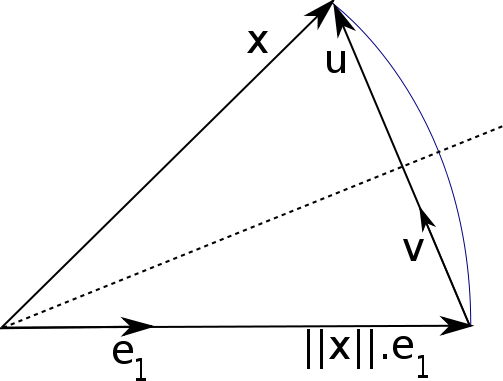
\includegraphics[scale=0.5]{./archivos/graficos/householder.png}
\end{center}

El objetivo es hallar una transformación lineal que cambie el vector $x$ en un vector de la misma longitud que sea colineal con $e_1$. Householder refleja a través de la línea punteada (elegida para dividir el ángulo entre $x$ y $e_1$). El máximo ángulo con esta transformación es a lo sumo de 45º.

Veamos un paso del procedimiento para poder ilustrar mejor: Sea $A \in \mathbb{R}^{n \times n}$ y sea $x_1$ el vector correspondiente a la primer columna de $A$ y $e_1$ el vector canónico, definimos:

\[
  \alpha_1 = \vectornorm{x_1}
\]
\[
  u = x_1 - \alpha_1 e_1
\]
\[
  v = \frac{u}{\vectornorm{u}}
\]
\[
  Q_1 = I - 2vv^{T}
\]

Luego $Q_1$ es la matriz que al multiplicarla a izquierda por $A$ coloca ceros por debajo de la diagonal.

\[
  Q_1A = \begin{bmatrix}
   \alpha_1&\star&\dots&\star\\
      0    &     &     &    \\
   \vdots  &     &  A' &    \\
      0    &     &     & \end{bmatrix}
\]

Repitiendo estos pasos: $Q_{n - 1} \dots Q_2Q_1A = R$. Luego el producto de las $Q$'s forma una matriz ortogonal, lo cual hace fácil y rápido hallar el vector solución del sistema.
\[
  Q^T = Q_{n - 1} \dots Q_2Q_1
\]
\[
  Ax = b \iff Q^TAx = Q^Tb \iff Rx = Q^Tb
\]

